\section{I Dataset}
Spesso nella tesi useremo il termine \textbf{dataset} ("insieme di dati" in italiano). 
Questo termine viene utilizzato per riferirsi ad una collezione 
strutturata di dati, generalmente di grandi dimensioni e organizzata, correlati a 
un argomento, tema o settore specifico. 

I dataset possono includere diversi tipi di informazioni, come numeri, testo, 
immagini, video e audio, e possono essere archiviati in vari formati, 
come CSV, JSON, SQL o altri formati.

I dataset possono essere utilizzati per condurre ricerche di mercato, 
analizzare i concorrenti, confrontare i prezzi, identificare e studiare le 
tendenze o addestrare modelli di apprendimento automatico. Questi sono solo 
alcuni esempi e i dataset sono utili in varie aree e situazioni. Ad esempio, noi 
utilizzeremo dei dataset per "addestrare" delle reti neurali per uno specifico 
problema \cite{Dataset_Bright,Dataset_Wikipedia}.
\newpage
\subsection{Tipologie di dataset per il ML}
Quando si addestra un modello di ML, vengono utilizzati diversi dataset per 
applicazioni differenti \cite{UTILIZZI_DATASET}:

\begin{itemize}
    \item \textbf{Training Dataset}: è il dataset utilizzato per addestrare il 
    modello di Machine Learning. Durante questa fase, il modello apprende le 
    relazioni e i pattern nei dati.

    \item \textbf{Validation Dataset}: è utilizzato per monitorare il modello 
    durante l'addestramento e ridurre il rischio di overfitting, ovvero quando 
    il modello si adatta troppo bene ai dati di addestramento e 
    perde capacità di generalizzare.
    
    \item \textbf{Test Dataset}: è il dataset utilizzato dopo l'addestramento per 
    valutare le prestazioni finali del modello. Serve a confermare 
    che il modello generalizzi bene su dati completamente nuovi.
\end{itemize}

Questi dataset possono essere anche ottenuti partendo da uno stesso dataset, 
dividendo il dataset principale in diversi dataset più piccoli.
Tipicamente, dal dataset principale, si utilizza un 60-70\% per il training, un 10-20\% 
per la validation e un 10-20\% per il test \cite{DIVISIONE_DATASET,DIVISIONE_DATASET_2}.

\begin{figure}[H]
    \centering
    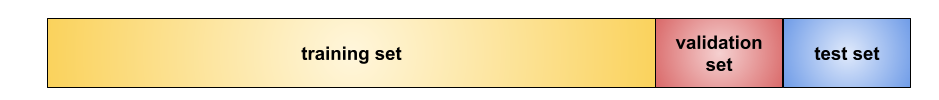
\includegraphics[width=1\textwidth]{Immagini/Generiche/PartitionThreeSets.png}
    \caption{Rappresentazione della suddivisione del dataset \cite{DIVISIONE_DATASET}.}
\end{figure}
